\documentclass{article}
\usepackage{graphicx}
\begin{document}
\title{Stable Marriage}
\author{Jinfeng Lin}
\maketitle
\clearpage
\section{Homework Exercise}
\subsection{Exercise 3.12}
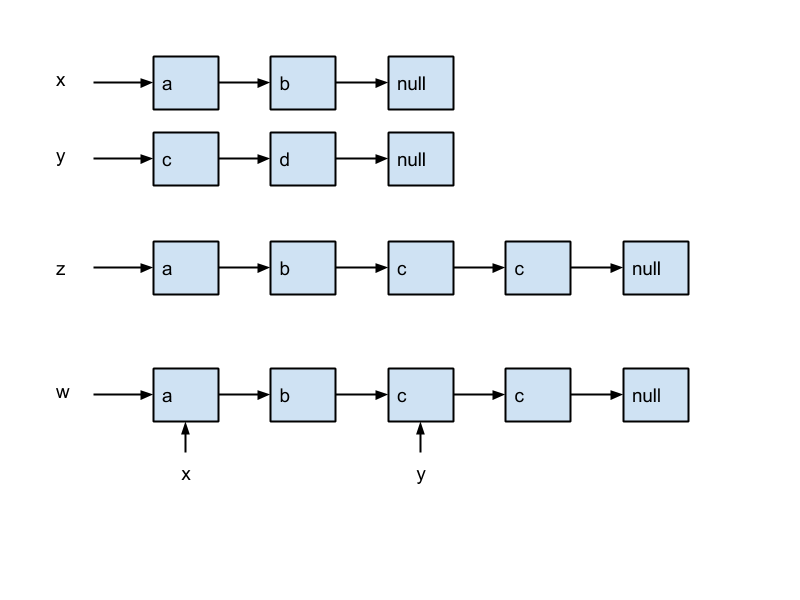
\includegraphics[width=\textwidth]{./figure}
\indent \par The first (cdr x) will get the rest of ('a 'b) after chopping the 'a off, because append generate z while keep x intact. When we do (cdr x) after append!, x is changed, the last element, which is null, is replaced by y, so when we do second cdr, x is ('a 'b 'c 'd).
\subsection{Exercise 3.14}
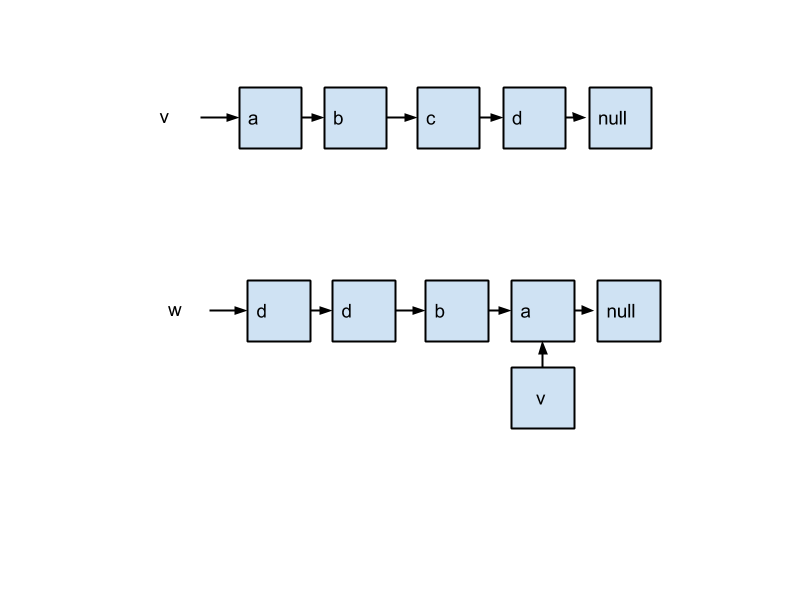
\includegraphics[width=\textwidth]{./figure2}
\indent \par This function reversed the input array v. The first one is v before the mystery operation, the following one is what w and v looks like after mystery function. The v become a pair ('a '()) at the first call of mystery.
\subsection{Exercise 3.17}
See in the code. By adding the  check process in control flow it is able to handle infinite loop. Because once a pair is inside it means its subcomponents are also inside the memory, we could spare time for searching them. That's why we could avoid the loop.
\section{The Algorithm}
\section{Implementation of People}
\subsection{Problem 0}
\indent \par According to my understanding, the cases actually is hidden in the iterations. The case described in document include 'Engaged received more than one proposal' and 'Unengaged received more than one proposal'. In the scheme code, actually each person will deal with one proposal at a time, the best one will be stored inside data structure, so inside the data structure, there is a condition clause to see if that person is engaged or not, if it is then compare the current one with the new proposer. The case-like pattern is replaced by multiple times of comparing between new proposer and current-indented.
\subsection{Problem 1}
See in code
\subsection{Problem 2}
See in code
\subsection{Problem 3}
See in code
\subsection{Problem 4}
Assume proposer M is not engaged after the algorithm and there are totally N pair of people. Then the rest N-1 proposers are engaged with N-1 proposees. It means there is at least 1 proposee is not engaged, even N-1 subset is stable, this proposee will proposer M. Then The assumption is not correct, all proposer will be engaged.
\subsection{Problem 5}
\indent \par In the first round every proposer will propose to the woman he love most, the ones failed will go to the next round, the ones succeed will be engaged. In the next round, the proposers will could only propose to the ones he love less because if he propose to the former one he will still be denied. If he succeed he may move another proposer to the unengaged set, and these ones could only propose to less like one otherwise will be denied again.
\indent \par For the proposees, in the first round if they are not engaged, they accept any one, if they are engaged only if the second proposer has higher order in preference, otherwise will all denied. In the following rounds, only higher order proposers will be accepted, others will all be denied.
\subsection{Problem 6}
\indent \par The inside mechanism for stable mechanism is that for each pair couple, man propose to women by the preference order, once it is accepted and not dumped at the end, it prove he is best proposers among any former proposer who have ever proposed to that woman.
\indent \par Let's assume the proposer m love w more than his wife and w love m more than his husband. Then in the begin, w will propose to m before his current wife, then no matter m's husband has proposed or not, w will replace m's current husband , because m accept the higher order one.
\indent \par The reason why m and w are not together is that before m propose to w, here is another women whose order is higher than w, and at the same time m is the highest order one among her proposers. If m proposed to his wife, it means he has failed on the women who have higher order than his wife. His wife is the best mate he could get. 
\indent \par So the conclusion is that, if m love w more, while at the mean time they are not couple, it means w loves her husband more; if w loves m more while they are not couple, it means w don't have chance to propose to her, because his wife has  higher order, he love his wife more than w.
\subsection{Problem 7}
\indent The men get engaged with the girl he love most, while the women don't, at the mean time the marriage is stable. So it indicates to be a proposer would have more advantage than waiting be to proposed.
\end{document}